\documentclass{article}

% if you need to pass options to natbib, use, e.g.:
% \PassOptionsToPackage{numbers, compress}{natbib}
% before loading nips_2017
%
% to avoid loading the natbib package, add option nonatbib:
% \usepackage[nonatbib]{nips_2017}

% to compile a camera-ready version, add the [final] option, e.g.:
\usepackage[final]{nips_2018}

\usepackage[utf8]{inputenc} % allow utf-8 input
\usepackage[T1]{fontenc}    % use 8-bit T1 fonts
\usepackage{hyperref}       % hyperlinks
\usepackage{url}            % simple URL typesetting
\usepackage{booktabs}       % professional-quality tables
\usepackage{amsfonts}       % blackboard math symbols
\usepackage{nicefrac}       % compact symbols for 1/2, etc.
\usepackage{microtype}      % microtypography
\usepackage{amsmath}
\usepackage{amssymb}
\usepackage{algorithmicx,algorithm,eqparbox,array}
\usepackage[noend]{algpseudocode}
\usepackage{graphicx}

\title{Learning Traveling Salesperson Routes with Graph Neural Networks}

\author{
  Marcelo Prates\thanks{Equal conttribution} \\
  Institute of Informatics\\
  Federal University of Rio Grande do Sul\\
  Porto Alegre, Brazil \\
  \texttt{morprates@inf.ufrgs.br} \\
  \And
  Pedro Avelar{$^*$} \\
  Institute of Informatics\\
  Federal University of Rio Grande do Sul\\
  Porto Alegre, Brazil \\
  \texttt{pedro.avelar@inf.ufrgs.br} \\
  \And
  Luis Lamb \\
  Institute of Informatics\\
  Federal University of Rio Grande do Sul\\
  Porto Alegre, Brazil \\
  \texttt{lamb@inf.ufrgs.br} \\
  }

\makeatletter
\def\BState{\State\hskip-\ALG@thistlm}
\makeatother

\algnewcommand{\LineComment}[1]{\State // #1}

\graphicspath{{figures/}}

\begin{document}

\maketitle

\begin{abstract}
\end{abstract}

\section{Introduction}

\section{Motivation}

Graph Neural Networks (GNNs) have been applied to a wide range of relevant problems [citations needed]. Very interesting recent work has shown how GNNs can be employed to bridge the divide between the neural and symbolic schools of artificial intelligence. In particular, \cite{selsam2018learning} has succeeded in training a GNN as a boolean satisfiability (SAT) predictor by feeding it CNF formulas as features and satisfiability bits (one per formula) as labels, thus learning a rudimentary SAT solver from single-bit supervision. The ``neurosat'' architecture, as the authors call it, is rather simple: it consists of assigning a multidimensional embedding $\in \mathbb{R}^d$ for each literal (i.e. $x_3$, $\neg x_1$, $x_{10}$, etc.) and each clause in a CNF formula and then connecting these embeddings accordingly so that they can send messages to one another -- literals are connected with the clauses in which they appear and vice-versa, and each literal is also connected to its negated variant (i.e. $x_1$ and $\neg x_1$). The model is run for a given number of message passing iterations in which each node in the GNN (i.e. a literal or a clause) adds up element-wise all of the embeddings of its incoming messages, received along its adjacencies, to obtain an accumulated message. The main trainable component of this architecture is a recurrent unit assigned with updating the embedding of a node with this accumulated message. In a nutshell, neurosat iterates a process of ``embedding refinement'' in which literals and clauses become enriched with information about their symbolic neighborhood. After that, each refined literal embedding is translated (by the means of a multilayer perceptron) into a logit probability, all of which are averaged to produce a final satisfiability prediction.

The success story of neurosat is an invitation to assess whether similar performance can be obtained for other $\mathcal{NP}$-Hard problems. Graph problems are suitable candidates, as they fit nicely into the relational structure of GNNs. The Traveling Salesperson Problem (TSP), assigned with finding the shortest length Hamiltonian path in a graph (that which visits each vertex exactly once), is a natural choice given its last longing relevance to computer science. Studying GNN models for TSP has another advantage: it allows us to assess whether GNNs can tackle problems where the connections between elements are labeled with numerical information -- in our case, edges carrying differing weights.

\section{Our Model}

Typical GNN architectures link adjacent vertices in the graph $\mathcal{G} = (\mathcal{V}, \mathcal{E})$ which represents the problem instance by opening a direct communication channel between their corresponding embeddings, in such a way that one can send messages to the other. Concretely, if we picture the collection of all $|\mathcal{V}|$ vertex embeddings at time $t$ as a matrix $\mathbf{V}^t \in \mathbb{R}^{|\mathcal{V}| \times d}$, the process of filtering the incoming messages for each node corresponds to performing a matrix multiplication with the graph's adjacency matrix, $\mathbf{M}$. Then the process of refining all embeddings at once can be expressed by Equation \ref{eq:refining_node_embeddings}, where $\mathbf{V}_u$ is a recurrent unit and $\mathbf{V}_h^t \in \mathbb{R}^{|\mathcal{V}| \times d}$ is a matrix in which each line $\mathbf{V}_h^t[i]$ contains the hidden state, at time t, corresponding to the i-th vertex.

\begin{equation} \label{eq:refining_node_embeddings}
\mathbf{V}_h^{t+1}, \mathbf{V}^{t+1} \leftarrow V_u( \mathbf{V}_h^t, \mathbf{M} \times \mathbf{V}^t )
\end{equation}

However one can see that this approach fails when connections are augmented with some numerical information such as edge weights or capacities. To feed this information into the network, we propose a new architecture which elevates edges to a ``node'' status in the context of the GNN. Concretely, we will assign embeddings to both vertices and edges, and link the embedding of each edge $e=(v_1,v_2)$ with the embeddings of the two vertices it connects ($v_1$ and $v_2$). The importance of having edge embeddings is that now we can feed them their ``labels'' (i.e. edge weights, edge capacities, etc.) at each message-passing timestep.

In this context, our neural algorithm includes $t_{max}$ message-passing iterations, each of which is composed of two steps: a vertices refinement step and an edges refinement step (Lines \ref{alg:line:vertices_refinement} and \ref{alg:line:edges_refinement} of Algorithm \ref{alg:GNN-TSP} respectively). Each vertex $v$ has its embedding refined upon feeding the recurrent unit $V_u$ with 1) the combined messages received from all the edges $(v,v',w) \in \mathcal{E}$ in which $v$ appears as a source vertex and 2) the combined messages received from all the edges $(v',v,w) \in \mathcal{E}$ in which $v$ appears as a target vertex. Each edge $e = (v_1, v_2, w)$ has its embedding refined upon feeding the recurrent unit $E_u$ with 1) one message received from $v_1$ 2) one message received from $v_2$ and 3) a scalar message containing the numerical value of $w$.

Note that because vertex embeddings are updated given two distinct element-wise sums of messages $\in \mathbb{R}^d$, the recurrent unit $V_u$ receives inputs $\in \mathbb{R}^{2d}$. Analogously, the recurrent unit $E_u$ receives inputs $\in \mathbb{R}^{2d+1}$ because of the extra scalar. These recurrent units are main trainable components of our model, learning to do the most important work: refine embeddings by compiling relational data.

Some attention must be given to the components $E_{msg}$ and $V_{msg}$, which are also trainable. Because the learned projections from vertices and edges to d-dimensional space is expected to be very different, we include two multilayer perceptrons (MLPs) assigned with translating edge embeddings to vertex embeddings ($E_{msg}$) and vertex embeddings to edge embeddings ($V_{msg}$).

The final trainable component of our model is $E_{vote}$, a MLP assigned with translating edge embeddings into logit probabilities, which we interpret as how certain the network is that each edge belongs to the optimal TSP route.

\begin{algorithm}[H]
\caption{Graph Neural Network TSP Solver}\label{alg:GNN-TSP}
\begin{algorithmic}[1]
\Procedure{GNN-TSP}{$\mathcal{G} = (\mathcal{V},\mathcal{E})$}

\State {\small Enumerate the edges of the graph, assigning an unique index $\mathcal{E}_{idx}[(v_1,v_2,w)]$ for each edge $(v_1,v_2,w) \in \mathcal{E}$}
\State
\LineComment{{\small Compute adj. matrix from edges to source vertices}}
\State $\mathbf{M_{EV_{src}}}[e,v] \leftarrow 1 \textrm{ if } \exists v' (\mathcal{E}_{idx}[(v,v')] = e) ~|~ \forall e \in \{1 \dots |\mathcal{E}|\}, \forall v \in \{1 \dots |\mathcal{V}|\}$
\LineComment{{\small Compute adj. matrix from edges to target vertices}}
\State $\mathbf{M_{EV_{tgt}}}[e,v] \leftarrow 1 \textrm{ if } \exists v' (\mathcal{E}_{idx}[(v',v)] = e) ~|~ \forall e \in \{1 \dots |\mathcal{E}|\}, \forall v \in \{1 \dots |\mathcal{V}|\}$ 
\LineComment{{\small Compute edge weights vector}}
\State $\mathbf{W}[\mathcal{E}_{idx}[(v_1,v_2,w)]] \leftarrow w ~|~ \forall (v_1, v_2, w) \in \mathcal{E}$ 
\State
\LineComment{Run $t_{max}$ message-passing iterations}
\For{$t=1 \dots t_{max}$}
  \LineComment{{\small Refine each vertex embedding with messages received from all the edges in which it appears}}
  \LineComment{{\small either as a source or a target vertex}}
  \label{alg:line:vertices_refinement}\State $\mathbf{V}_h^{t+1}, \mathbf{V}^{t+1} \leftarrow V_u( \mathbf{V}_h^t, \mathbf{M_{EV_{src}}} \times E_{msg}(\mathbf{E}^t), \mathbf{M_{EV_{tgt}}} \times E_{msg}(\mathbf{E}^t) )$
  \LineComment{{\small Refine each edge embedding with (two) messages received from its source and its target vertex}}
  \label{alg:line:edges_refinement}\State $\mathbf{E}_h^{t+1}, \mathbf{E}^{t+1} \leftarrow E_u( \mathbf{E}_h^t, \mathbf{M_{EV_{src}}}^{T} \times V_{msg}(\mathbf{V}^t), \mathbf{M_{EV_{tgt}}}^{T} \times V_{msg}(\mathbf{V}^t), \mathbf{W} )$
\EndFor
\State
\LineComment{{\small Translate edge embeddings into logit probabilities}}
\State $E_{logits} \leftarrow E_{vote}(E^{t_{max}})$
\LineComment{{\small Convert logit probabilities into probabilities}}
\State $E_{prob} \leftarrow sigmoid(E_{logits})$
\LineComment{{\small Extract route}}
\State $Route \leftarrow \{ (v_1,v_2,w) ~|~ (v_1,v_2,w) \in \mathcal{E}, E_{prob}[\mathcal{E}_{idx}[(v_1,v_2,w)]] > 0.5 \}$
\EndProcedure
\end{algorithmic}
\end{algorithm}

\subsection{Training}
\label{sub:training}

The most natural way to train this model is to perform stochastic gradient descent on the binary cross entropy loss between the computed edge probabilities and an ``edges mask'' with ones in the indices corresponding to edges in the solution and zeros elsewhere. This training, of course, has the disadvantage of requiring a rather large amount of labels ($|\mathcal{E}|$). We can also anticipate a problem: if the training instances were to allow multiple optimal TSP routes, the network would not be able to choose the same route we compute, as we are required to break ties through some arbitrarily chosen criterion (such as lexicographic ordering of vertices). As we will see in the ``Results and Analysis'' section, this is actually the case: unable to choose between two routes of similar or equal cost, the trained model resorts to outputting a superposition of good quality routes. Hopefully, this issue can be treated with a simple fix: we can compute a ``degree loss'' which penalizes nodes with in and out degrees $\neq 1$. This is similar to a flow conservation constraint in the context of Integer Linear Programming (ILP). This can be done by computing two tensors, $\overline{\textrm{deg}^{+}}$ and $\overline{\textrm{deg}^{-}}$, of expected in and out degrees for each vertex, respectively. Concretely, we define:

\begin{equation}
\begin{aligned}
\overline{\textrm{deg}^{+}} \leftarrow & \left(M_{EV_{src}}\right)^T \times E_{prob} \\
\overline{\textrm{deg}^{-}} \leftarrow & \left(M_{EV_{tgt}}\right)^T \times E_{prob} \\
loss(\textrm{deg}^{-}) \leftarrow & \sum~(\overline{\textrm{deg}^{-}}-1)^2 \\
loss(\textrm{deg}^{+}) \leftarrow & \sum~(\overline{\textrm{deg}^{+}}-1)^2 \\
loss(\textrm{deg}) \leftarrow & ~loss(\textrm{deg}^{+}) + loss(\textrm{deg}^{-})
\end{aligned}
\end{equation}

And apply stochastic gradient descent on $loss(\textrm{deg})$ in addition to the binary cross entropy between the edges mask and the computed probabilities.

\section{Experimental Setup}

We produce training instances by sampling $n=20$ random points on a $\frac{\sqrt{2}}{2} \times \frac{\sqrt{2}}{2}$ square and filling a distance matrix $\mathbf{D} \in \mathbb{R}^{n \times n}$ with the euclidean distances between each pair of points (which by construction are $\in [0,1]$). We then quantize edge weights into $b=100$ different integer bins, producing $\mathbf{D}' = [b\mathbf{D}]$. For each such set of points we produce two complete graphs $\mathcal{G} = (\mathcal{V},\mathcal{E})$ and $\mathcal{G}_{int} = (\mathcal{V},\mathcal{E}_{int})$ where $\mathcal{V} = \{v_1, \dots, v_n\}$, $\mathcal{E} = \{(v_i,v_j,\frac{1}{b}\mathbf{D}'[i,j]) ~|~ v_i \in \mathcal{V}, v_j \in \mathcal{V}\}$ and $\mathcal{E}_{int} = \{(v_i,v_j,\mathbf{D}'[i,j]) ~|~ v_i \in \mathcal{V}, v_j \in \mathcal{V}\}$. Because $\mathcal{G}$ and $\mathcal{G}_{int}$ identical up to scale, their optimal TSP tours are guaranteed to be the same. Finally, we solve the TSP problem on $\mathcal{G}_{int}$ using Google's Operations Research Tools \cite{or-tools-user-manual} and feed $\mathcal{G}$ to our model as a training instance.

We produce $4096$ such instances, grouping them in batches of $32$. Note that instances can be easily batched by performing a disjoint union over a set of graphs $\{\mathcal{G}_{1} = (\mathcal{V}_1,\mathcal{E}_1), \dots \mathcal{G}_{n} = (\mathcal{V}_n,\mathcal{E}_n)\}$: 

\begin{equation}
\mathcal{G}_U = \bigcup_{i=1}^{n}{\mathcal{G}_i} = \left(\bigcup_{i=1}^{n}{\mathcal{V}_i}, \bigcup_{i=1}^{n}{\mathcal{E}_i}\right)
\end{equation}

To produce our features and performing a disjoint union over a set of tours \\ $\{ T_1 \in \mathcal{E}^{|\mathcal{V}_1|}, \dots, T_n \in \mathcal{E}^{|\mathcal{V}_n|} \}$:

\begin{equation}
T_U = \bigcup_{i=1}^{n}{T_i}
\end{equation}

To produce our labels. At each batch (from $128$ total) we perform a SGD iteration on both the binary cross entropy between the edges mask and the computed edge probabilities and the ``degree loss'' defined in Section \ref{sub:training}.

\begin{figure}[H]
  \centering
  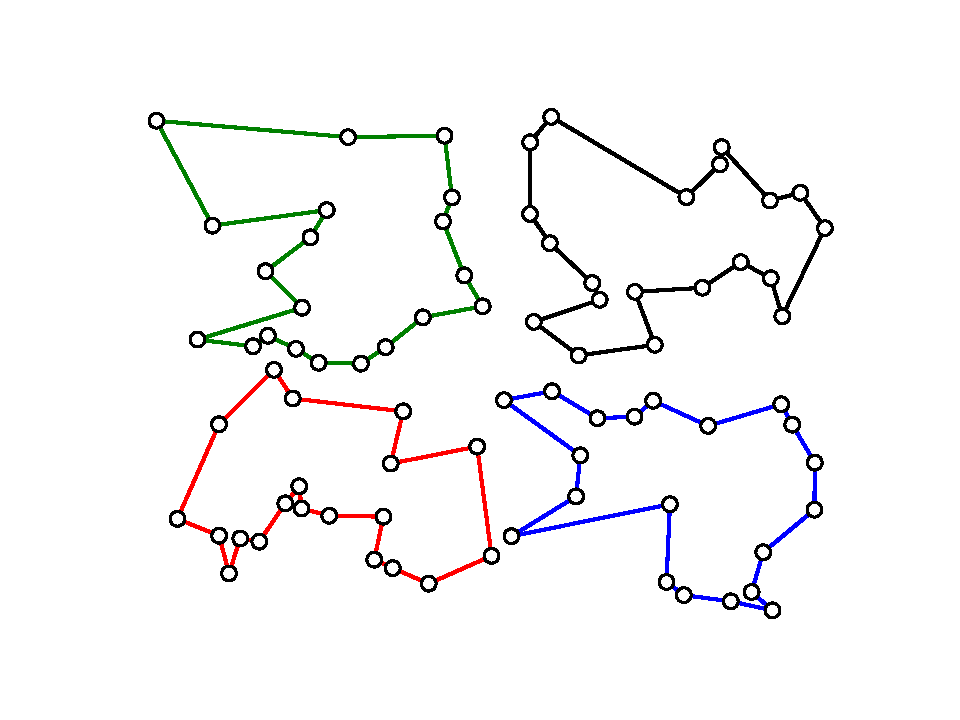
\includegraphics[width=\linewidth]{training-inst-examples.pdf}
  \caption{Examples of graphs produced as training instances, with the associated optimal TSP tours painted in different colors.}
  \label{fig:training-inst-examples}
\end{figure}

\section{Results and Analysis}

\section{Discussion}

\bibliographystyle{named}
\bibliography{bib}

\end{document}